\documentclass[]{article}

\usepackage{amsmath}
\usepackage{graphics}
%I'd like to know a bit more about the experiments - I guess these are
%sections 5.2/3/4.  Would you be able to give me a brief summary of
%these, say a page each: the RQ being addressed, the methodology, and
%what the results would look like (metrics, tables, graphs etc.).

%opening
\title{Thesis Experiments}
\author{Andrew Healy}

\begin{document}

\maketitle

For the following experiments, the provers under consideration are Z3, Alt-Ergo, CVC3, CVC4, Yices, veriT. The sets \emph{training} and \emph{test} are disjoint subsets of the 919 individual proof obligations generated by Why3 from the 117 example WhyML programs included in the standard Why3 distribution. The independent/predictor variables are various metrics statically derived from the proof obligation goals: number of operators, number of variables, number of constants etc. The dependent/repsponse variables are the \emph{time} taken by each prover (measured in seconds) and the \emph{result} returned by Why3. These were dynamically measured with a statistical confidence interval of 90\%. The ratio of the size of the training set to the test set is approximately 3:1.
\vspace{0.4cm}

\textit{Null hypothesis:}

\textbf{Static metrics derived from proof obligation goals do not indicate the performance of any SMT prover.} 

\section{Predicting Prover Result}


Given the set of possible prover results 
\[ 
 Res = \lbrace Valid, Invalid, Unknown, Timeout, Error \rbrace
\]
Can the correct prover result $r \in  Res$ be predicted for an arbitrary proof obligation $p \in training$ for each prover?

\subsection{Research Questions addressed}
\label{rq1}
\begin{itemize}
\item{Can the single most effective solver for a Why3 proof obligation be predicted by learning from static metrics?}
\item{Can a useful ranking of solvers be predicted for a Why3 proof obligation?}
\end{itemize}

\subsection{Methodology}

\textbf{Data preprocessing:} Perform standard scaling of the independent/predictor variables in \emph{training}. Call this matrix $X$
\label{preprocess}

Whether the procedure below is implemented separately for each prover depends on whether the learning algorithm supports multivariate output (e.g. Decision Trees) or not (e.g Support Vector classifiers). 

\begin{enumerate}
\item{Separate \textit{result} columns from \textit{time} of the dependent/response variables in \textit{training}. Call this matrix $y$}
\item{Fit the classification model on $X$ and $y$}
\item{For each proof $p$ obligation in \textit{testing}:}
\begin{itemize}
	\item[a.] Scale $p$'s independent/predictor variables with the scaler used in step 1.
	\item[b.] Predict the result $r$ on the model
\end{itemize}
\end{enumerate}

\subsection{Evaluation}
\label{eval1}
We will compare our classifier against \textbar$Res$\textbar dummy classifiers: that is, $\mathcal{CLF}_{r}$ will always choose result $r$ for each proof obligation in $testing$.  
The evaluation of multiclass classification where the class weights are not balanced (i.e. we have far more \textit{Valid} responses in \textit{training} than \textit{Error}, thankfully) can be given with the \textbf{Weighted Empirical Error}: Let $W_c$ be the weight of the class $c$. Set the weights such that $\frac{1}{W_c} \sim \frac{1}{n} \sum_{i \leq n} 1_{c_i = c}$ and define the weighted empirical error
\[
	err_W(g) = \frac{1}{n} \sum_{i \leq n} W_{c_i} 1_{g(x_i) \neq c_i}
\]

Another evaluation metric for multiclass classification is the  \textbf{Receiver Operating Characteristic} (ROC). This is a plot of the rate of false positives against the rate of false negatives for each class. Commonly used for evaluating binary classifications, it can be extended to the multiclass case by computing the mean of the scores for each class (fig: \ref{fig:roc}). Our classes would be $Res$. steeper curves (approaching the top left) and a higher \textbf{Area Under Curve} (AUC) scores  are better: they show a low false positive rate and high true positive rate.   

\begin{figure}[h!]
	\scalebox{0.5}{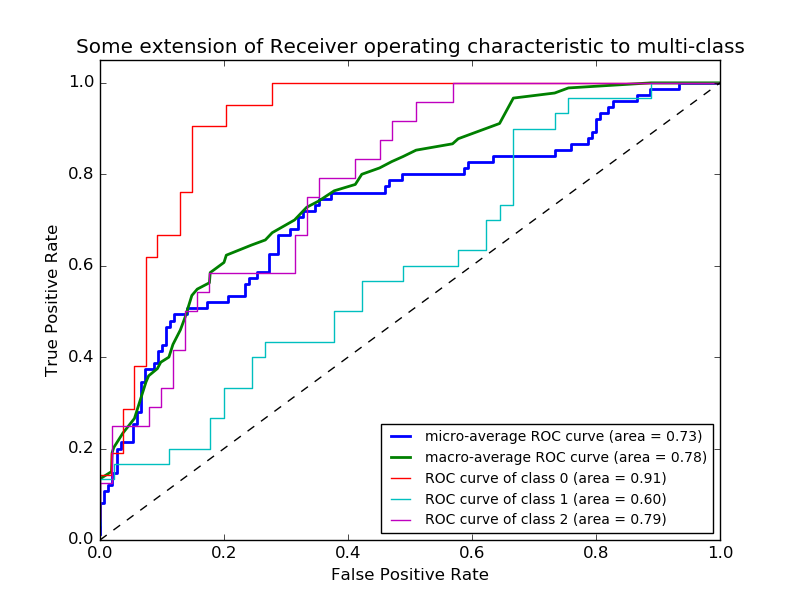
\includegraphics{plot_roc_002.png}}
	\caption{Example ROC plot for multiclass classification: taken from $http://scikit-learn.org/stable/auto\_examples/model\_selection/plot\_roc.html$}
	\label{fig:roc}
\end{figure}

\section{Predicting Prover Time}

Can the time a prover takes to return a result be accurately predicted for an arbitrary proof obligation $p \in training$ for each prover?

\subsection{Research Questions addressed}
(same as \ref{rq1})

\subsection{Methodology}

$time$ is a continuous-valued variable measured in seconds generally in the range $\lbrack 0.001, 12.3 \rbrack$ (depending on the prover's interaction with Why3). There are a number of possibities for predicting this variable - either attempting to predict it directly as a regression task or by treating it as a classification task by the approximating the actual values into discrete bins. Each have their distinct methodolgies but share the same initial data preprocessing step (as in section \ref{preprocess})

\subsubsection{Regression}

\begin{enumerate}
\item{Separate \textit{time} columns from \textit{result} of the dependent/response variables in \textit{training}. Call this matrix $y$}
\item[2-3.]{Same as steps 2-3 in section \ref{preprocess}; replacing classification with regression to predict $time$}
\end{enumerate} 

\subsubsection{Binary Classification}
\label{binary}

The rationale behind treating this as a binary classification problem is that by inspecting the timings for each prover, it is clear that the vast majority of results are returned in a very short amount of time (\textit{Valid}, \textit{Invalid} or instantly \textit{Unknown}, probably), or close to the timeout value (\textit{Timeout} and a large proportion of \textit{Unknown} and \textit{Error} results).

\vspace{0.2in}

\noindent\fbox{%
    \parbox{\textwidth}{%
        \textbf{Data preprocessing: (in addition to section \ref{preprocess})} \\ For the vector $T$ of $time$ reponses for each prover:
    
        a. Define $lo$ as the 0.25 quartile of $T$ and $hi$ as the 0.75 quartile. 
        
        b. $t' = 
        \begin{cases} 
        hi,&\text{if }t > mean(T) \\
        lo,&\text{otherwise}
        \end{cases}$ 
        
        c. $y$ is the vector of binarized $t'$ times  
    }%
}
\vspace{0.2in}

Otherwise the methodolgy is the same as section \ref{preprocess} with the result being the predicted $time$ (which will be one of each prover's $hi$ or $lo$ values).

\subsubsection{Multiclass Classification}

Increasing the number of bins from 2 gives a better chance of returning an accurate result through classification.

\vspace{0.2in}

\noindent\fbox{%
    \parbox{\textwidth}{%
        \textbf{Data preprocessing: (in addition to section \ref{preprocess})}
              
        a. Bin the values in $time$ so that each bin has an approx. equal number of values and the number of bins does not exceed 5 (to increase the liklihood of accurate predictions)
        
        b. Assign each value to it's corresponding bin
        
        c. $t' = mean( bin_{t} )$  
        
        c. $y$ is the vector of discretised $t'$ times  
    }%
}
\vspace{0.2in}

(same as section \ref{preprocess} - with the result being the mean of the predicted bin)

\subsection{Evaluation}

\subsubsection{Regression}
\label{eval2}

A number of metrics to evaluate regression models can handle the multi-output case. An average of the error for all outputs is returned. In our case, the output is a vector of reals corresponding to out set of provers. 
\begin{itemize}
\item{The \textbf{Mean Squared Error}  determines the squared difference between the predicted value and the actual value.}
\item{The \textbf{$R^{2}$ Score} (also called the coefficient of determination) is a measure of how well the model is expected to predict future values. It takes into account the variance of the dependent/response variables.}
\end{itemize}

We will compare our regressor to a dummy regressor which always returns the mean of $time$.
 
\subsubsection{Binary and Multiclass Classification}

We can use all the metrics from sections \ref{eval1} and \ref{eval2} to end up with a table similar to Table \ref{table:exp2}. Here, $hi$, $lo$, Bins1-3 are dummy classifiers whose predicted constants can be used for regression metrics and as labels for classification metrics.+

\begin{table}
\centering
\caption{Evaluation of using 3 methods to predict time (with dummy values apart from \textbf{Actual} row. Note that the Classification metrics cannot be used for the reggressors)}\label{table:exp2}
\begin{tabular}{r||r|r||r|r} %\hline
& \textbf{AUC}& \textbf{Weighted Emp. Err.}& \textbf{Mean Sq. Err.} & \textbf{$R^{2}$ Score}\\ \hline
\textbf{Actual} & 1.0  & 0.0 & 0.0 & 1.0  \\ \hline \hline
\textbf{Regressor}& - & - & 0.5 & 0.7\\ \hline
mean & - & - & 0.7 & 0.3\\ \hline \hline
\textbf{Binary} & 0.5 & 0.4 & 0.4 & 0.6\\ \hline
$lo$& 0.2 & 0.6 & 0.6 & 0.5\\ \hline
$hi$ & 0.2 & 0.6 & 0.6 & 0.5\\ \hline \hline %\hline
\textbf{3-bins} & 0.7 & 0.3 & 0.3 & 0.8\\ \hline 
Bin1 & 0.3 & 0.7 & 0.7 & 0.4\\ \hline
Bin2 & 0.3 & 0.7 & 0.7 & 0.4\\ \hline
Bin3 & 0.3 & 0.7 & 0.7 & 0.4\\
\end{tabular}
\end{table}


 



\end{document}
